%2multibyte Version: 5.50.0.2953 CodePage: 65001
\documentclass[11pt,letter]{article}%
\usepackage{float}
\usepackage{amsmath}
\usepackage{amsfonts}
\usepackage{amssymb}
\usepackage{rotating}
\usepackage{graphicx}
\usepackage{subcaption}
\usepackage{color}
\usepackage{booktabs}
\usepackage{standalone}
\usepackage[height=9in,left=1in,right=0.75in,bottom=1in]{geometry}
\usepackage[breaklinks=true,bookmarksopen=true,colorlinks=true,citecolor=blue]%
{hyperref}
\usepackage{epstopdf}
\usepackage[authoryear]{natbib}
%\usepackage{subfig}
\usepackage{threeparttable}
\usepackage{multirow}
\usepackage{listings}%
\usepackage[inline]{enumitem}
\setcounter{MaxMatrixCols}{30}
\providecommand{\U}[1]{\protect\rule{.1in}{.1in}}
%EndMSIPreambleData
\newtheorem{theorem}{Theorem}
\newtheorem{acknowledgement}{Acknowledgement}[section]
\newtheorem{algorithm}{Algorithm}[section]
\newtheorem{axiom}{Axiom}[section]
\newtheorem{case}{Case}[section]
\newtheorem{claim}{Claim}[section]
\newtheorem{conclusion}{Conclusion}[section]
\newtheorem{condition}{Condition}[section]
\newtheorem{conjecture}{Conjecture}[section]
\newtheorem{corollary}{Corollary}[section]
\newtheorem{criterion}{Criterion}[section]
\newtheorem{definition}{Definition}[section]
\newtheorem{example}{Example}[section]
\newtheorem{exercise}{Exercise}[section]
\newtheorem{lemma}{Lemma}
\newtheorem{notation}{Notation}[section]
\newtheorem{problem}{Problem}[section]
\newtheorem{proposition}{Proposition}
\newtheorem{remark}{Remark}[section]
\newtheorem{solution}{Solution}[section]
\newtheorem{summary}{Summary}[section]
\newenvironment{proof}[1][Proof]{\noindent\textbf{#1.} }{\ \rule{0.5em}{0.5em}}
\renewcommand{\baselinestretch}{1.3}
\newcommand{\oops}{\color{red}\textbf{$<$file does not exist$>$}\color{black}}
\usepackage{tikz}
\usepackage{color,soul}
\usepackage{caption}
\usepackage{pgfplots}
\usepackage[utf8]{inputenc}

\makeatletter
\numberwithin{equation}{section}

% Cross-ref
\usepackage{xr}


% Souting text
%\usepackage[normalem]{ulem}

\begin{document}

\title{\textbf{Community Detection in A Network of Money Circulation}}
\author{Juan Estrada\thanks{Department of Economics, Emory University, Ph.D. Student in economics. E-mail: \href{mailto:juan.jose.estrada.sosa@emory.edu}{jjestra@emory.edu}.}\and Diego Rojas\thanks{Department of Economics, Emory University, Ph.D. Student in economics. E-mail: \href{diego.israel.rojas.baez@emory.edu}{drojasb@emory.edu}.}\and Yinghui Dong\thanks{Department of Computer Science, Georgia Institute of Technology, Ms.c. Student in computer science.}}
\date{\today}

\maketitle 

\lstset{language=,numbers=left, numberstyle=\tiny, stepnumber=1, numbersep=5pt,moredelim=[is][\ttfamily]{|}{|}}

\begin{abstract}
	\noindent Community detection has proved to be one important tool for the description of different types of network structures. From the economics perspective, understanding social architecture is a key piece in the analysis of observed outcomes across different markets. Social relevance and data availability, have facilitated the existence of new bigger network datasets. This poses big challenges for the scalability of existing algorithms. This paper joins the economic and computational perspectives. From one side, we implement an efficient algorithm to cluster network data when additional nodes characteristics are observed. We show the behavior of the algorithm using different simulated datasets, parameters, and intermediate optimization methods. The results show that the algorithm is able to find the cluster structure when the rank reduction parameter is known. On the other hand, we apply the clustering algorithm to the network of money circulation in Canada. The results show that the clustering structure is noticeably sensitive to the change in the rank reduction parameter.
\end{abstract}

\section{Introduction}

Network structures shape the observed outcomes across different types of markets. Human behavior like crime, substances abuse, educational achievement among others is significantly affected by social interactions. More complex structures developed by individuals including financial systems are also governed by network architecture. The importance of networks in determining market outcomes is translated into an empirical relevance of understanding what characteristics of the network are relevant. In this regard, community detection has become a key task from both the social and computational perspectives \citep{Jackson2019,Du2017}. 

One particular market where the network structure is a cause and a consequence of human social interaction is the market of money circulation in a country. If we think about the economic structure of a nation as a human body, bank bills are comparable with the red blood cells in the human circulatory system. This analogy leads to an important implication: understanding bills' individual behavior will enlighten the mechanisms determining the operation of the complete economic system. This article is divided into two main components. The initial part of the paper presents the implementation of the algorithm developed by \cite{Du2017b}. In this section, we provide a test for the performance of the algorithm using a simulated data set. Additionally, we show differences in complexity when changing the way how the minimization problems are calculated. In the second part of the article, we use the developed algorithm to perform a clustering procedure to the network of money circulation in Canada. This method allows us to find existing communities in the network while also using important observable characteristics of the bank notes (bank notes and notes are going to be used as interchangeably).

In particular, this document uses the Information Management System Program study of bank notes from the Bank of Canada (BoC). This is a unique data set containing records that track the events in the ``life'' of every note issued by the Bank of Canada. For this document, we have a sample of around 300 million note scan records. The period for which data is obtained is the year from August 2017 to July 2018. We can build networks at two levels:  the region level and the financial institutions level networks. Specifically, the financial institution that receives the note from the Bank, and the financial institution that deposits back the note are known.  

The most attractive feature of this analysis is that the richness of the data allows to observe the circulation patterns of every single note existing in the Canadian economy. The paper focuses on the network spanned by the circulation of the notes across regions and financial institutions to perform the community detection exercise. 


\section{Related work}

This article can relate with two different literatures. From the computational perspective, this article belongs to the literature of community detection methods. A well structured summary of the development of methods of community detection can be found in \cite{Du2017}. The authors present a complete review regarding joint matrix factorization. The method implemented in this paper has multiple advantages over previous approaches. It improves how interpretable are the matrix resulting from the proposed decomposition. Additionally, it overcomes some computationally difficulties based on the non-negative constrain of all factors. In the same vein, there have been developments regarding clustering methods, \cite{2018CCod} present a relevant work with the advantage of including clustering of directed graphs.

From the perspective of community detection in backing, the literature is not developed yet. Theoretically, the detection of existent communities is relevant because of the possibility of contagion of idiosyncratic shocks through the network structure in the financial system \citep{Gai2010}. Related with the existence of communities is the density of the connection for some particular subgraphs of the total network and it may also enhances financial stability \citep{acemoglu2015}. Despite the theoretical contributions regarding the importance of communities to predict financial stability, to our knowledge, there are not empirical papers developing banking community detection. Our paper contributes to fill the gap of empirical evidence of the existence of financial communities in the network of money circulation.

\section{The problem and context}

As mentioned, the goal of the paper is to efficiently perform a community detection of a network dataset containing additional information of the nodes. To achieve the objective, we implement the hybrid clustered algorithm developed by \cite{Du2017}. For this paper, we have information of the principal financial institutions in Canada. For those institutions we can observe an identifier of the bank receiving transfers of bank notes from the Bank of Canada. Analogously, we observe the financial institution that deposits back the bank notes. With this information, we define a connection between two financial institutions \textit{A} and \textit{B} as a situation where \textit{Bank A} receives the note $x$ from the Bank of Canada which is followed by \textit{Bank B} depositing the same note back to the Bank of Canada. Each connection between two financial institutions varies in the amount of bank notes that are received and deposited. This yields a network of size 50. Note that this definition generates a directed network because the number of notes sent from Bank \textit{A} to \textit{B} may be different from the number sent from Bank \textit{B} to \textit{A}.

The algorithm in \cite{Du2017} is designed for symmetric adjacency matrices. To create a symmetric matrix, we redefine the connections as the total amount of transactions between banks \textit{A} and \textit{B}. For each bank note, we have a total of 25 fit characteristics, 5 denominations, and we can observe whether the bill was transfer or deposited to the BoC. Utilizing notes' characteristics, we create aggregate features for each financial institution. To capture the possible heterogeneity in bank notes' fit, we use the 10 deciles of the empirical distribution of fit characteristics within each financial institution instead of just the sample means. This procedures give us a total of 3,350 observable characteristics for each bank. Therefore, our matrix of observable information is defined by $X \in \mathbb{R}_{+}^{m \times n}$ and the graph structure is represented the symmetric matrix $S \in \mathbb{R}_{+}^{n \times n}$ where $m=2,200$ and $n=50$. The objective is to find a low rank representation that simultaneously account for the network structure and the characteristics matrix information. The objective function formalizing this idea is given by:

\begin{equation}
\min\limits_{W\geq 0,H \geq 0} ||X-WH||^{2}_{F}+\alpha||S-H^{T}H||^{2}_{F},
\label{e3}
\end{equation}

where $\alpha$ is the weighting parameter, $W \in \mathbb{R}_{+}^{m \times k}$ and $H \in \mathbb{R}_{+}^{k \times n}$ where $k$ is much smaller than $m$ and $n$. The article propose a block coordinate descent (BCD) scheme to find the solution for the objective function which require to solve the following three subproblems:

\begin{align}
\label{e4}
&\min\limits_{W\geq 0} ||H^{t}W^{t}-X^{t}||_{F} \\
\label{e5}
&\min\limits_{\tilde{H}\geq 0} \left\Vert \begin{bmatrix}\sqrt{\alpha}H^{t}  \\ \sqrt{\beta} I_k \end{bmatrix} \tilde{H} - \begin{bmatrix}\sqrt{\alpha}S  \\ \sqrt{\beta} H \end{bmatrix}\right\Vert_{F}\\
\label{e6}
&\min\limits_{\tilde{H}\geq 0} \left\Vert \begin{bmatrix} W \\ \sqrt{\alpha} \tilde{H}^{t} \\ \sqrt{\beta} I_k \end{bmatrix} H - \begin{bmatrix} X \\ \sqrt{\alpha} S \\ \sqrt{\beta} \tilde{H} \end{bmatrix}\right\Vert_{F}.\\
\end{align}

Note that each subproblem is a nonnegative least squares (NLS). The procedure is based on an iterative algorithm that has been proved to converge. The solution of the NLS can be based on different basic decompositions. In the next sections, we show that the algorithm that implement works for a testing data set, we change the basic decomposition and show how the performance of the algorithm change, and finally we apply it to our empirical dataset.  

\section{Algorithm Performance}

As mention in Section 3, the objective of the algorithm is find the solution of Equation \ref{e3} which can be done solving the subproblems in \ref{e4}, \ref{e5} and \ref{e6}. As each problem is a NLS we can apply different methods to solve each minimization problem. To test the code, we will use simulated data with fixed seed. First, we define $m$, $n$ and $k$ and randomly generate $W$ and $H$. Then, using this random matrices, we create $X=WH$ and $S=H^{T}H$. For this test we set $\alpha=\beta=1$. We compare three different methods to solve the minimization problem, namely normal equations, active set and block pivot. We vary the size of the matrices $X$ and $S$ and compare the results of each method. 

\begin{table}[H]
	\centering
	\caption{Comparison of the methods}
	\label{t1}
	\begin{tabular}{lllccc}
	\hline
	\multicolumn{3}{c}{Parameters} &	Normal Equations	&	Active Set	&
	Block Pivot	\\
	\hline
	m=200	&	n=100	&	k=4	&	0.35	&	1.98	&	0.91	\\
	m=200	&	n=1,000	&	k=4	&	4.8	&	3.8	&	3.9	\\
	m=200	&	n=10,000	&	k=4	&	42	&	212	&	14.3	\\
	m=2,000	&	n=1,000	&	k=4	&	8.8	&	5.4	&	5.1	\\
	m=20,000	&	n=1,000	&	k=4	&	8	&	38.3	&	34.7	\\
	m=2,000	&	n=1,000	&	k=10	&	14.7	&	10.9	&	5.9	\\
	m=2,000	&	n=1,000	&	k=20	&	23.3	&	63	&	7.2	\\
	m=2,000	&	n=1,000	&	k=40	&	43	&	222	&	13.7	\\
	\hline
\end{tabular}		
\end{table}

Table \ref{t1} presents the results in time for each of the methods varying the parameters determining the size of each matrix. It shows that in general, when the size of the matrices is increased, Block Pivot has a better performance than the other methods. This simulation confirms the expected results regarding the complexity of the algorithms \citep{kim2008}.  

\section{Results}

As previously stated we have developed a two stage strategy to use the algorithm. In first place we simulate data from randomly generated matrices to resemble perfectly clustered data. This allows us to test the performance of the clustering method to detect communities. In second place we use the real data obtained describing the paths followed by notes issued by the Bank of Canada. This paths span a network where the vertices are the financial institutions in each region of Canada.

\subsection{Test  Data}

In order to test the data we had to come up with a minimal working example that the algorithm would always be able to replicate. In the case this particular  community detection algorithm we reversed engineered the process of decomposition. 

First, notice that the number of rows of the matrix $H$, is the number of possible clusters where every vertex can be assigned. From a hard clustering perspective, a vertex belongs to the community, i.e. row, where it shows the largest value. In other words the $i$-th observation will belong to the cluster $j$-th if the $H_{ij}\geq H_{ij'}$, for all $j'$. 

Therefore, the minimal working example can be built by simulating a matrix $H$ that presents perfect clustering. In other words, that each column of  $H$ is full of zeroes with the exception of the row that shows the membership of the vertex to a particular cluster. The structure of $W$ is not particularly important for the simulation as long as the matrix is somewhat dense. 

Based on the simulated matrix $\widetilde{H}$ we can build the matrices $X=\widetilde{W}\widetilde{H}$ and  $S=\widetilde{H}^T\widetilde{H}$. These matrices can be fed to the algorithm to test how the algorithm performs under known perfect clustering. For this example the simulated network $X$ has dimensions $n=500$ and $m=10.000$. This achieved by simulating a $\widetilde{H}$ matrix with $k$ rows and $500$ columns.  For this simulation we have choose $k=6$ for the sake of illustration. However, the choice of $k$ under this simulation framework is not relevant as long as we work under the assumption that the number communities is known. 



\begin{figure}[!h]
    \centering
    \begin{subfigure}[b]{0.45\textwidth}
            \centering
            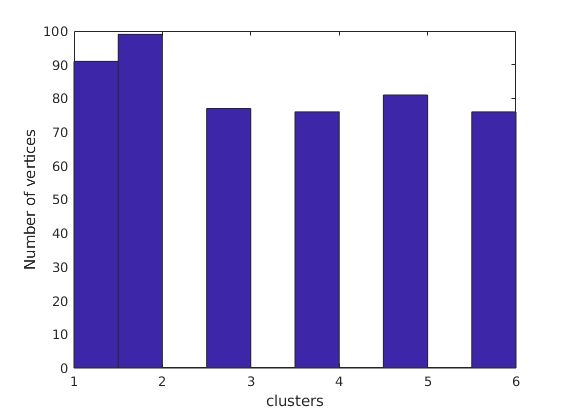
\includegraphics[width=\textwidth]{../original_6.png}
    \label{fig:fig1}
    \end{subfigure}
\begin{subfigure}[b]{0.45\textwidth}
            \centering
            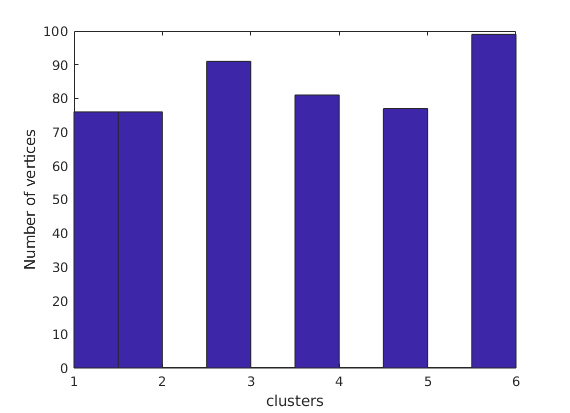
\includegraphics[width=\textwidth]{../estimated.png}
    \label{fig:fig2}
    \end{subfigure}
    \caption{\protect\subref{fig:fig1}, The left panel  shows the clustering structure of the simulated data. On the  right panel, \protect\subref{fig:fig2} we observe the number of vertices by cluster estimated by the algorithm}
\end{figure}

The results obtained by the simulation showed two consistent behaviors. First, the number of clusters is replicated precisely when the correct $k$ is provided to the algorithm. While the labeling of the cluster might change neither the number of clusters, nor the cluster membership change from the simulated data to the estimated by the algorithm. In other words, this estimation is equivalent up to relabeling of clusters. This becomes evident when observing Figure 1. Each one of the columns in the graph represent the number of vertices that are included in each one of the six clusters. Is evident from the comparison of panels that each column in the graph on the left panel can be matched, in absolute value, to a column on the right panel, however the label of the cluster changes.

The important takeaway from the simulation is the sensitivity of the $k$ parameter. Changing the number of clusters can really affect the structure of the communities identified. In this particular case, a deviation to a value of $k=8$ caused the  algorithm to become unstable. A choice of $k=5$ changed fundamentally the structure of the clusters. In general with other simulations is clear that the algorithm can be unstable when deviating from the true $k$. 



\begin{figure}[!h]
    \centering
    \begin{subfigure}[b]{0.45\textwidth}
            \centering
            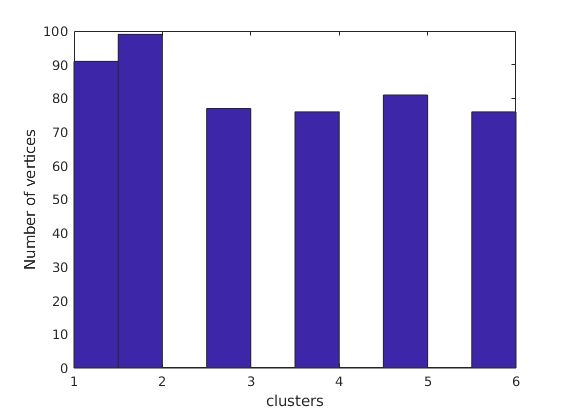
\includegraphics[width=\textwidth]{../original_6.png}
    \label{fig:fig1}
    \end{subfigure}
\begin{subfigure}[b]{0.45\textwidth}
            \centering
            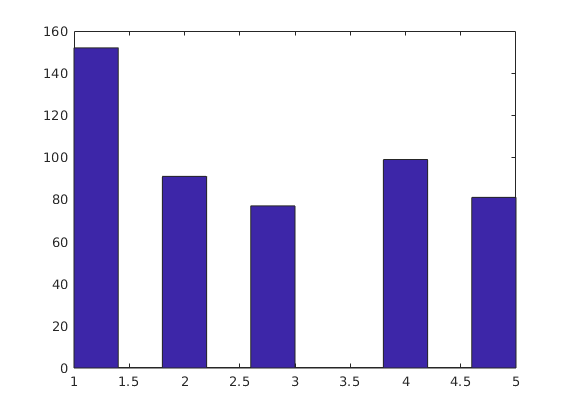
\includegraphics[width=\textwidth]{../kmis.png}
    \label{fig:fig2}
    \end{subfigure}
    \caption{\protect\subref{fig:fig1}, The left panel  shows the clustering structure of the simulated data. On the  right panel, \protect\subref{fig:fig2} we observe the number of vertices by cluster estimated by the algorithm when the parameter $k=5$}
\end{figure}

Is important to notice, that the conclusions drawn using the extreme, hard clustering, scenario also hold under a more relaxed structure of $H$\footnote{Several such simulations have been run by the authors, these can be found in the appended code}.


\subsection{Results: A network of money}


Given the good performance of the algorithm under ideal conditions, the logical next step is to implement the network data. The size of the original data set made it impossible to process such data under \textit{MATLAB}, hence the preparation of the original matrices had to be done with both \textit{Python} and \textit{Postgresql}. 

\begin{figure}[!h]
    \centering
    \begin{subfigure}[b]{0.45\textwidth}
            \centering
            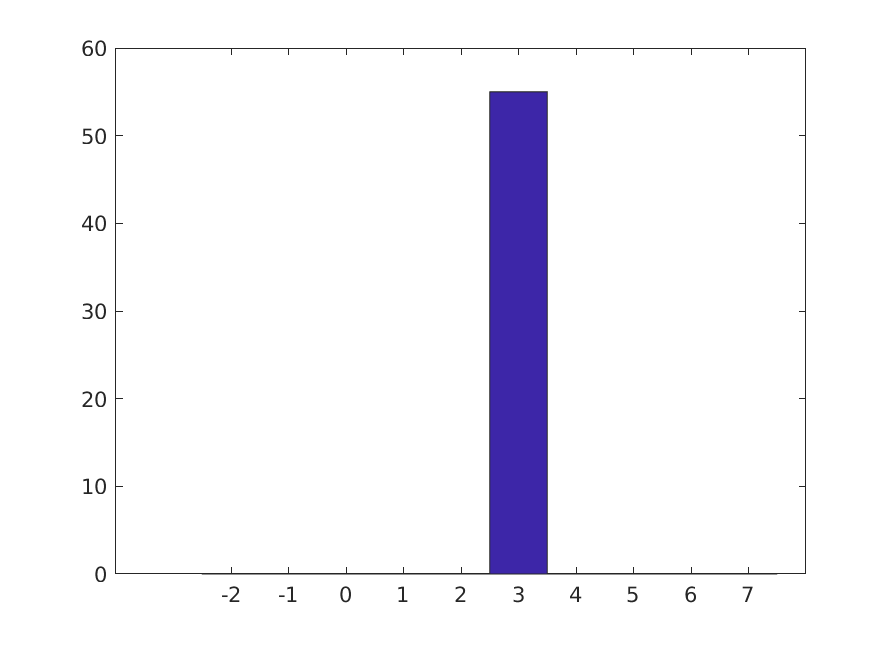
\includegraphics[width=\textwidth]{../FIG1.png}
    \label{fig:fig1}
    \end{subfigure}
\begin{subfigure}[b]{0.45\textwidth}
            \centering
            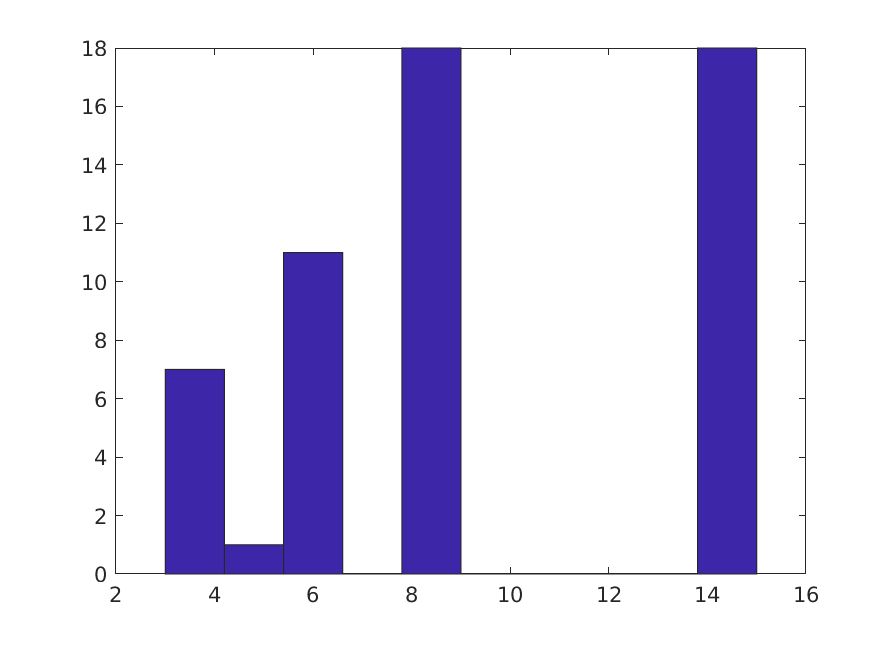
\includegraphics[width=\textwidth]{../FIG2.png}
    \label{fig:fig2}
    \end{subfigure}
    \begin{subfigure}[b]{0.45\textwidth}
            \centering
            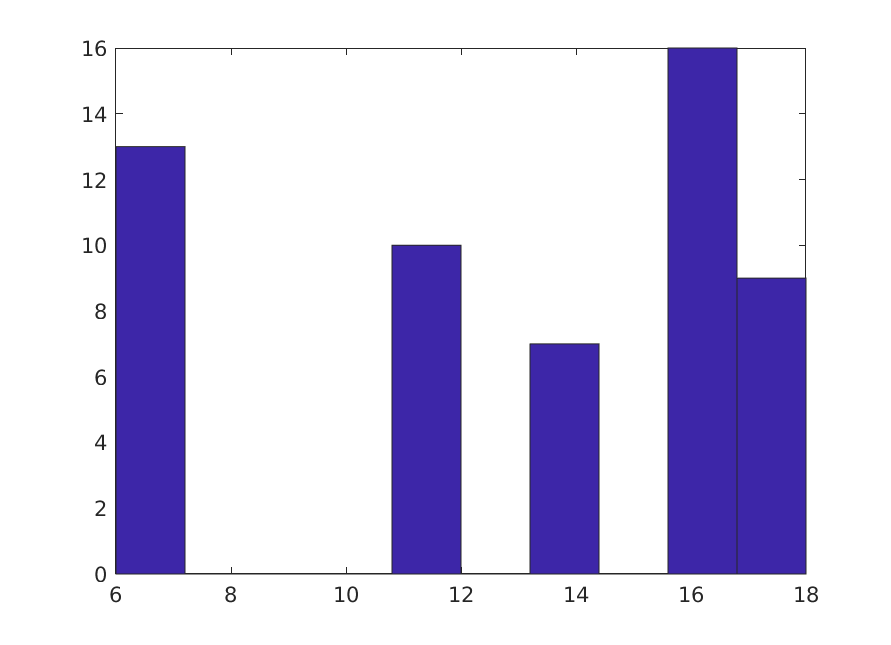
\includegraphics[width=\textwidth]{../FIG3.png}
    \label{fig:fig3}
    \end{subfigure}
    \begin{subfigure}[b]{0.45\textwidth}
            \centering
            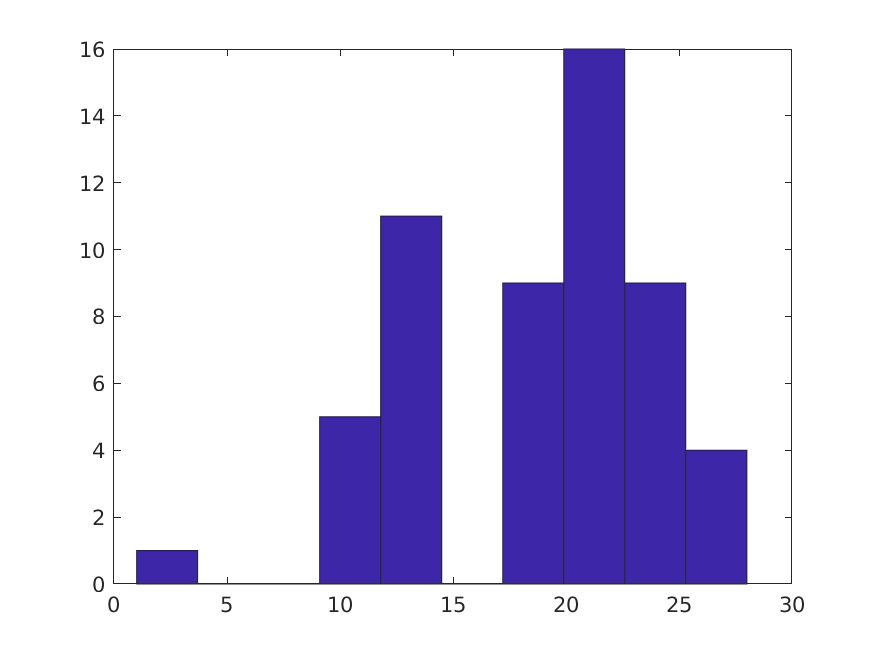
\includegraphics[width=\textwidth]{../FIG4.png}
    \label{fig:fig4}
    \end{subfigure}
    \caption{\protect\subref{fig:fig1} The left upper panel shows the clustering structure of the simulated data under $k=10$. The left upper panel shows the clustering structure of the simulated data under $k=15$. The left upper panel shows the clustering structure of the simulated data under $k=20$. The left upper panel shows the clustering structure of the simulated data under $k=30$.}
\end{figure}

The results are certainly astonishing. For the sake of transparency, we run the algorithm for the real data, constructed as described in section 2, for several choices of rank $k$. We observed that for $10> k\geq1$  the number of clusters is equal to one and the algorithm successfully assigning every vertex to a cluster. The number of clusters increases gradually as the choice of $k$ increases, however, there is no $k<50$ for which the number of clusters fully matches the number of rows of $H$. This happens despite the fact that for every clustering structure all of the vertex are assigned unambiguously to one of the clusters. Meaning, the load of $H_{ij}$ for the particular cluster of the $i$-th observation is considerably higher to the loads of other clusters. This result is also persistent despite the number of iterations that we allow the algorithm to run.

This opens the question of how is that this results comes to be and whether such clustering is an appropriate description of how communities form in such a network. From this exercise, we can conclude that while the algorithm is successful in approximating the equations described in the problem statement, the number of clusters end up not being the same as the rank specified for the rank reduced decomposition.  Further inquiry in this matter is recommended. 

\section{Conclusions}

This paper successfully implement the efficient algorithm for hybrid clustering developed by \cite{Du2017}. We show via simulation that the implemented algorithm is able to capture the existing clusters when the number for rank reduction is known. Additionally, in the simulations we show that the method is highly sensitive to changes in the parameter $k$. In the second part of the paper we apply the clustering algorithm to the network of money circulation in Canada. The conclusion after the exerciser is that, as expected, we need a valid criteria to define $k$.  That is because when changing this parameters, the clustering results considerably differ. From the empirical perspective, the application of algorithm to the data left us with the important research question: how can we determine a valid value $k$ for a particular observable data? 

\bibliographystyle{abbrv}
\bibliography{refrences}\clearpage

\end{document}